% Options for packages loaded elsewhere
\PassOptionsToPackage{unicode}{hyperref}
\PassOptionsToPackage{hyphens}{url}
%
\documentclass[
]{book}
\usepackage{amsmath,amssymb}
\usepackage{lmodern}
\usepackage{iftex}
\ifPDFTeX
  \usepackage[T1]{fontenc}
  \usepackage[utf8]{inputenc}
  \usepackage{textcomp} % provide euro and other symbols
\else % if luatex or xetex
  \usepackage{unicode-math}
  \defaultfontfeatures{Scale=MatchLowercase}
  \defaultfontfeatures[\rmfamily]{Ligatures=TeX,Scale=1}
\fi
% Use upquote if available, for straight quotes in verbatim environments
\IfFileExists{upquote.sty}{\usepackage{upquote}}{}
\IfFileExists{microtype.sty}{% use microtype if available
  \usepackage[]{microtype}
  \UseMicrotypeSet[protrusion]{basicmath} % disable protrusion for tt fonts
}{}
\makeatletter
\@ifundefined{KOMAClassName}{% if non-KOMA class
  \IfFileExists{parskip.sty}{%
    \usepackage{parskip}
  }{% else
    \setlength{\parindent}{0pt}
    \setlength{\parskip}{6pt plus 2pt minus 1pt}}
}{% if KOMA class
  \KOMAoptions{parskip=half}}
\makeatother
\usepackage{xcolor}
\usepackage{color}
\usepackage{fancyvrb}
\newcommand{\VerbBar}{|}
\newcommand{\VERB}{\Verb[commandchars=\\\{\}]}
\DefineVerbatimEnvironment{Highlighting}{Verbatim}{commandchars=\\\{\}}
% Add ',fontsize=\small' for more characters per line
\usepackage{framed}
\definecolor{shadecolor}{RGB}{248,248,248}
\newenvironment{Shaded}{\begin{snugshade}}{\end{snugshade}}
\newcommand{\AlertTok}[1]{\textcolor[rgb]{0.94,0.16,0.16}{#1}}
\newcommand{\AnnotationTok}[1]{\textcolor[rgb]{0.56,0.35,0.01}{\textbf{\textit{#1}}}}
\newcommand{\AttributeTok}[1]{\textcolor[rgb]{0.77,0.63,0.00}{#1}}
\newcommand{\BaseNTok}[1]{\textcolor[rgb]{0.00,0.00,0.81}{#1}}
\newcommand{\BuiltInTok}[1]{#1}
\newcommand{\CharTok}[1]{\textcolor[rgb]{0.31,0.60,0.02}{#1}}
\newcommand{\CommentTok}[1]{\textcolor[rgb]{0.56,0.35,0.01}{\textit{#1}}}
\newcommand{\CommentVarTok}[1]{\textcolor[rgb]{0.56,0.35,0.01}{\textbf{\textit{#1}}}}
\newcommand{\ConstantTok}[1]{\textcolor[rgb]{0.00,0.00,0.00}{#1}}
\newcommand{\ControlFlowTok}[1]{\textcolor[rgb]{0.13,0.29,0.53}{\textbf{#1}}}
\newcommand{\DataTypeTok}[1]{\textcolor[rgb]{0.13,0.29,0.53}{#1}}
\newcommand{\DecValTok}[1]{\textcolor[rgb]{0.00,0.00,0.81}{#1}}
\newcommand{\DocumentationTok}[1]{\textcolor[rgb]{0.56,0.35,0.01}{\textbf{\textit{#1}}}}
\newcommand{\ErrorTok}[1]{\textcolor[rgb]{0.64,0.00,0.00}{\textbf{#1}}}
\newcommand{\ExtensionTok}[1]{#1}
\newcommand{\FloatTok}[1]{\textcolor[rgb]{0.00,0.00,0.81}{#1}}
\newcommand{\FunctionTok}[1]{\textcolor[rgb]{0.00,0.00,0.00}{#1}}
\newcommand{\ImportTok}[1]{#1}
\newcommand{\InformationTok}[1]{\textcolor[rgb]{0.56,0.35,0.01}{\textbf{\textit{#1}}}}
\newcommand{\KeywordTok}[1]{\textcolor[rgb]{0.13,0.29,0.53}{\textbf{#1}}}
\newcommand{\NormalTok}[1]{#1}
\newcommand{\OperatorTok}[1]{\textcolor[rgb]{0.81,0.36,0.00}{\textbf{#1}}}
\newcommand{\OtherTok}[1]{\textcolor[rgb]{0.56,0.35,0.01}{#1}}
\newcommand{\PreprocessorTok}[1]{\textcolor[rgb]{0.56,0.35,0.01}{\textit{#1}}}
\newcommand{\RegionMarkerTok}[1]{#1}
\newcommand{\SpecialCharTok}[1]{\textcolor[rgb]{0.00,0.00,0.00}{#1}}
\newcommand{\SpecialStringTok}[1]{\textcolor[rgb]{0.31,0.60,0.02}{#1}}
\newcommand{\StringTok}[1]{\textcolor[rgb]{0.31,0.60,0.02}{#1}}
\newcommand{\VariableTok}[1]{\textcolor[rgb]{0.00,0.00,0.00}{#1}}
\newcommand{\VerbatimStringTok}[1]{\textcolor[rgb]{0.31,0.60,0.02}{#1}}
\newcommand{\WarningTok}[1]{\textcolor[rgb]{0.56,0.35,0.01}{\textbf{\textit{#1}}}}
\usepackage{longtable,booktabs,array}
\usepackage{calc} % for calculating minipage widths
% Correct order of tables after \paragraph or \subparagraph
\usepackage{etoolbox}
\makeatletter
\patchcmd\longtable{\par}{\if@noskipsec\mbox{}\fi\par}{}{}
\makeatother
% Allow footnotes in longtable head/foot
\IfFileExists{footnotehyper.sty}{\usepackage{footnotehyper}}{\usepackage{footnote}}
\makesavenoteenv{longtable}
\usepackage{graphicx}
\makeatletter
\def\maxwidth{\ifdim\Gin@nat@width>\linewidth\linewidth\else\Gin@nat@width\fi}
\def\maxheight{\ifdim\Gin@nat@height>\textheight\textheight\else\Gin@nat@height\fi}
\makeatother
% Scale images if necessary, so that they will not overflow the page
% margins by default, and it is still possible to overwrite the defaults
% using explicit options in \includegraphics[width, height, ...]{}
\setkeys{Gin}{width=\maxwidth,height=\maxheight,keepaspectratio}
% Set default figure placement to htbp
\makeatletter
\def\fps@figure{htbp}
\makeatother
\setlength{\emergencystretch}{3em} % prevent overfull lines
\providecommand{\tightlist}{%
  \setlength{\itemsep}{0pt}\setlength{\parskip}{0pt}}
\setcounter{secnumdepth}{5}
\usepackage{booktabs}
\ifLuaTeX
  \usepackage{selnolig}  % disable illegal ligatures
\fi
\usepackage[]{natbib}
\bibliographystyle{apalike}
\IfFileExists{bookmark.sty}{\usepackage{bookmark}}{\usepackage{hyperref}}
\IfFileExists{xurl.sty}{\usepackage{xurl}}{} % add URL line breaks if available
\urlstyle{same} % disable monospaced font for URLs
\hypersetup{
  pdftitle={R Cookbook for Agricultural Research},
  pdfauthor={李誠紘 Cheng Hong, Li},
  hidelinks,
  pdfcreator={LaTeX via pandoc}}

\title{R Cookbook for Agricultural Research}
\author{李誠紘 Cheng Hong, Li}
\date{2022-12-08}

\begin{document}
\maketitle

{
\setcounter{tocdepth}{1}
\tableofcontents
}
\hypertarget{ux95dcux65bc}{%
\chapter{關於}\label{ux95dcux65bc}}

這是一本關於統計程式語言 R 的筆記,嘗試 (用白話文) 記錄我在 \textbf{農業試驗研究} 上使用的 R 程式語言。

\hypertarget{ux9019ux662fux4ec0ux9ebc}{%
\section{這是什麼?}\label{ux9019ux662fux4ec0ux9ebc}}

這是一個利用 \href{https://zh.wikipedia.org/wiki/R\%E8\%AF\%AD\%E8\%A8\%80}{R} bookdown 撰寫,部屬在Github Page上的電子書。

這是我的學習筆記、速查本。

這本書包含農業研究常用的統計學、試驗設計學、資料繪圖的 R 程式語言。

要讀懂這本書,基礎的試驗設計學知識是必須的。

\hypertarget{ux63a8ux85a6ux53c3ux8003ux8cc7ux8a0a}{%
\section{推薦參考資訊}\label{ux63a8ux85a6ux53c3ux8003ux8cc7ux8a0a}}

\begin{itemize}
\item
  \href{http://yijutseng.github.io/DataScienceRBook/index.html}{資料科學與R語言} by 長庚大學資管系曾意儒老師。中文版免費的R教科書。
\item
  \href{https://r4ds.had.co.nz/index.html}{R for Data Science} by Hadley Wickham and Garrett Grolemund。\href{https://hadley.nz/}{Hadley Wickham}是\href{https://posit.co/download/rstudio-desktop/}{RStudio}的科學家,也是R語言的耶穌。他寫出來的套件(packages)讓R語言變得更容易使用。這本書用生動有趣的文法介紹資料科學與R的好用套件。
\end{itemize}

本書的R語言版本:

\begin{Shaded}
\begin{Highlighting}[]
\FunctionTok{sessionInfo}\NormalTok{()}
\end{Highlighting}
\end{Shaded}

\begin{verbatim}
## R version 4.2.2 (2022-10-31 ucrt)
## Platform: x86_64-w64-mingw32/x64 (64-bit)
## Running under: Windows 10 x64 (build 19045)
## 
## Matrix products: default
## 
## locale:
## [1] LC_COLLATE=Chinese (Traditional)_Taiwan.utf8 
## [2] LC_CTYPE=Chinese (Traditional)_Taiwan.utf8   
## [3] LC_MONETARY=Chinese (Traditional)_Taiwan.utf8
## [4] LC_NUMERIC=C                                 
## [5] LC_TIME=Chinese (Traditional)_Taiwan.utf8    
## 
## attached base packages:
## [1] stats     graphics  grDevices utils     datasets  methods   base     
## 
## loaded via a namespace (and not attached):
##  [1] compiler_4.2.2  magrittr_2.0.3  fastmap_1.1.0   bookdown_0.30  
##  [5] cli_3.4.1       htmltools_0.5.3 tools_4.2.2     rstudioapi_0.14
##  [9] yaml_2.3.6      stringi_1.7.8   rmarkdown_2.18  knitr_1.40     
## [13] stringr_1.4.1   digest_0.6.30   xfun_0.34       rlang_1.0.6    
## [17] evaluate_0.18
\end{verbatim}

\hypertarget{ux958bux59cbux4e4bux524d}{%
\chapter{開始之前}\label{ux958bux59cbux4e4bux524d}}

事前作業:下載與安裝好 \href{https://cran.r-project.org/}{R} 及 \href{https://posit.co/download/rstudio-desktop/}{RStudio}

\begin{itemize}
\item
  R是必須要安裝的,否則沒辦法使用 (驚!!)
\item
  RStudio則是R語言的''整合開發環境'
  (Integrated Development Environment, IDE),讓你更舒服地撰寫程式。
\item
  雖說 RStudio 不是必須,但是本書程式碼全部都是在RStudio中寫出來的,可見 RStudio 有奪好用。
   
   
\end{itemize}

\hypertarget{ux7b2cux4e00ux500b-r-ux7a0bux5f0fux78bc}{%
\section{第一個 R 程式碼}\label{ux7b2cux4e00ux500b-r-ux7a0bux5f0fux78bc}}

複製下面程式碼,輸入 console 介面中,點按執行。

這是你的第一個R程式碼,哈囉世界!

\begin{Shaded}
\begin{Highlighting}[]
\FunctionTok{print}\NormalTok{(}\StringTok{\textquotesingle{}Hello world!\textquotesingle{}}\NormalTok{)}
\end{Highlighting}
\end{Shaded}

\begin{verbatim}
## [1] "Hello world!"
\end{verbatim}

 

本書會包含程式碼 (上方灰框) 與執行結果 (下方灰框),你可以直接複製貼上程式碼,在 R 介面中執行。
 

你會發現,\texttt{R語言}很像是Google助理,輸入一行指令,執行後就會返回一行結果。這種一來一往類型的程式語言叫做直譯語言 (Interpreted Language)。

但是,一段 R 的程式碼也有可能很多行,譬如下面畫圖的函數,就是一個多行組成的程式碼。
 
 

\hypertarget{ux7b2cux4e00ux5f35ux5716}{%
\section{第一張圖}\label{ux7b2cux4e00ux5f35ux5716}}

你可以將下面程式碼複製後,整個貼到你的RStudio介面或是R中執行,畫出你的第一張圖:

\begin{Shaded}
\begin{Highlighting}[]
\NormalTok{pkg }\OtherTok{\textless{}{-}} \StringTok{\textquotesingle{}ggplot2\textquotesingle{}}
\ControlFlowTok{if}\NormalTok{ ( pkg }\SpecialCharTok{\%in\%} \FunctionTok{installed.packages}\NormalTok{() }\SpecialCharTok{==} \ConstantTok{FALSE}\NormalTok{) }\FunctionTok{install.packages}\NormalTok{(pkg) }
\FunctionTok{invisible}\NormalTok{(}\FunctionTok{lapply}\NormalTok{(pkg, library, }\AttributeTok{character.only =} \ConstantTok{TRUE}\NormalTok{))}

\FunctionTok{ggplot}\NormalTok{(}\AttributeTok{data =}\NormalTok{ iris, }\AttributeTok{mapping =} \FunctionTok{aes}\NormalTok{(}\AttributeTok{x =}\NormalTok{ Sepal.Length, }\AttributeTok{y =}\NormalTok{ Petal.Width, }\AttributeTok{color =}\NormalTok{ Species))}\SpecialCharTok{+}
  \FunctionTok{geom\_jitter}\NormalTok{()}\SpecialCharTok{+}
  \FunctionTok{geom\_smooth}\NormalTok{(}\AttributeTok{method=}\StringTok{\textquotesingle{}lm\textquotesingle{}}\NormalTok{,}\AttributeTok{se=}\NormalTok{F)}\SpecialCharTok{+}
  \FunctionTok{theme\_bw}\NormalTok{()}\SpecialCharTok{+}
  \FunctionTok{labs}\NormalTok{(}\AttributeTok{x=}\StringTok{\textquotesingle{}花萼長度(cm)\textquotesingle{}}\NormalTok{,}
       \AttributeTok{y=}\StringTok{\textquotesingle{}花瓣寬度(cm)\textquotesingle{}}\NormalTok{,}
       \AttributeTok{color =} \StringTok{\textquotesingle{}品種\textquotesingle{}}\NormalTok{,}
       \AttributeTok{title =} \StringTok{\textquotesingle{}鳶尾花花萼長與花瓣寬線性關係\textquotesingle{}}\NormalTok{)}
\end{Highlighting}
\end{Shaded}

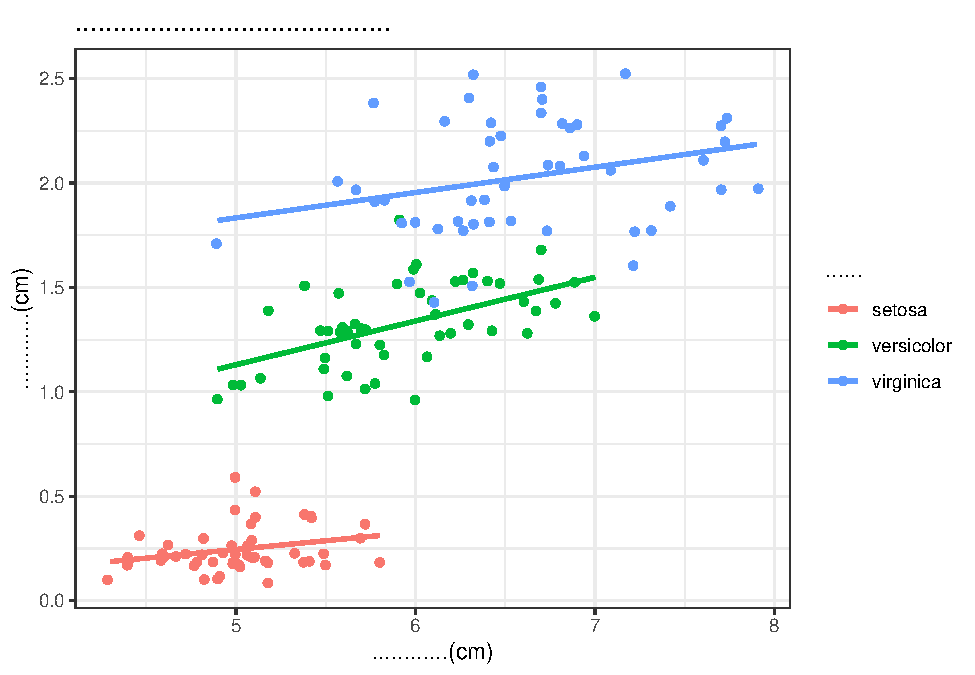
\includegraphics{_main_files/figure-latex/unnamed-chunk-4-1.pdf}

上面是利用R內建的資料\texttt{iris}所進行的繪圖,只要學會使用R語言,不同類型的資料也都可以畫出好看又專業的圖。

這筆資料又稱為鳶尾花(iris)資料集,是 R. A. Fisher 1938年出版的 \emph{The Use of Multiple Measurements in Taxonomic Problems} 中使用到的資料集。

這個資料集非常有名,包含有加拿大加斯帕半島採集到的三種鳶尾花品種形態資料。(葉茂生老師說:形不是型!不可以弄錯)

像這樣的資料集有非常多已經內建在R程式中,我們稱為\href{https://stat.ethz.ch/R-manual/R-devel/library/datasets/html/00Index.html}{範例資料集},可以用\texttt{data()}查看可利用那些資料。

\hypertarget{ux6558ux8ff0ux7d71ux8a08}{%
\chapter{敘述統計}\label{ux6558ux8ff0ux7d71ux8a08}}

這一章節的目的是介紹如何讀取資料,將資料進行簡單的統計量計算分析,例如平均值、樣本變異數、樣本數等等。

\hypertarget{ux8cc7ux6599ux683cux5f0f}{%
\section{資料格式}\label{ux8cc7ux6599ux683cux5f0f}}

統計分析的資料,以 Excel 檔整理成以下格式,並統一存成 UFT-8 編碼的 csv 檔。

csv 檔可以用 Excel 檔開啟,因此,一旦將寫在紙上的原始資料 (raw data) 輸入到 Excel 中,再轉存成 .csv檔,就可以直接由 R 讀取,相當方便。

\begin{figure}
\centering
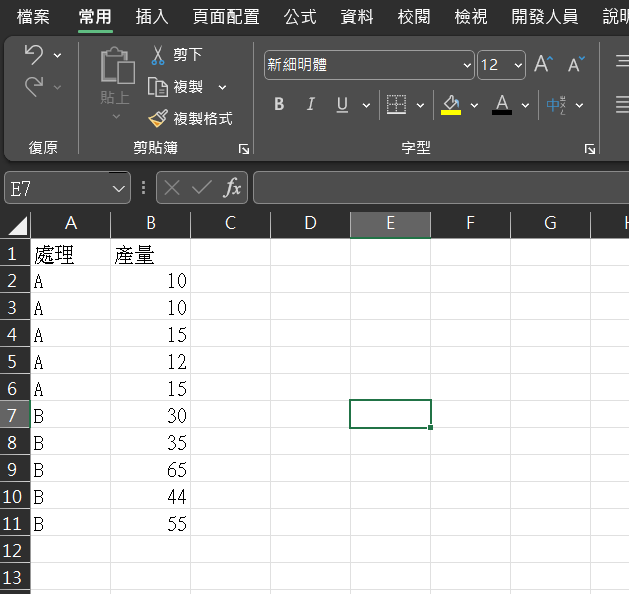
\includegraphics{image/excel.png}
\caption{R也看得懂的Excel表}
\end{figure}

這樣的資料在R裡面會長這樣(不建議資料表包含中文字元)

\begin{Shaded}
\begin{Highlighting}[]
\NormalTok{(df}\OtherTok{\textless{}{-}}\FunctionTok{data.frame}\NormalTok{(}
  \StringTok{\textquotesingle{}處理\textquotesingle{}} \OtherTok{=} \FunctionTok{rep}\NormalTok{(}\FunctionTok{c}\NormalTok{(}\StringTok{\textquotesingle{}A\textquotesingle{}}\NormalTok{,}\StringTok{\textquotesingle{}B\textquotesingle{}}\NormalTok{),}\AttributeTok{each=}\DecValTok{5}\NormalTok{),}
  \StringTok{\textquotesingle{}產量\textquotesingle{}} \OtherTok{=} \FunctionTok{c}\NormalTok{(}\DecValTok{10}\NormalTok{,}\DecValTok{10}\NormalTok{,}\DecValTok{15}\NormalTok{,}\DecValTok{12}\NormalTok{,}\DecValTok{15}\NormalTok{,}\DecValTok{30}\NormalTok{,}\DecValTok{35}\NormalTok{,}\DecValTok{65}\NormalTok{,}\DecValTok{44}\NormalTok{,}\DecValTok{55}\NormalTok{)}
\NormalTok{))}
\end{Highlighting}
\end{Shaded}

\begin{verbatim}
##    處理 產量
## 1     A   10
## 2     A   10
## 3     A   15
## 4     A   12
## 5     A   15
## 6     B   30
## 7     B   35
## 8     B   65
## 9     B   44
## 10    B   55
\end{verbatim}

上方印出的東西稱為資料表 (dataframe),資料表由2個變數 (variables) \texttt{處理}和\texttt{產量}組成。變數名稱所在的位置稱為欄位 (columns),欄位是有順序的,在上表中,第1欄為\texttt{處理}、第2欄為\texttt{產量}。每個欄位下面都有資料值 (values),稱為觀測值 (observations),觀測值左方的數字為列 (row) 數,可以看到這筆資料有2欄10列。

在開始前,請下載\href{}{\texttt{此檔案}},將其存放在 D 槽,以利後續分析。

\hypertarget{ux8b80ux53d6ux8cc7ux6599}{%
\section{讀取資料}\label{ux8b80ux53d6ux8cc7ux6599}}

使用\texttt{read.csv}函數

上方指令的意思是,讀取 csv 檔,檔案放在D槽底下,名稱為iris.csv (\texttt{file\ =\ \textquotesingle{}D:/iris.csv\textquotesingle{}}),而我想要幫這個資料表取名為\texttt{iris\_df}

箭頭 (\textless-) 在 R 中是代表賦值 (assign) 的操作子 (operator),意思是把''箭頭右方''的物件,放入''箭頭左方''的物件。

如果左方的物件沒有指派物件,左方物件就會變成箭頭右方物件的名字。(從今天開始你的代號就是9527!)

\begin{Shaded}
\begin{Highlighting}[]
\NormalTok{快龍的招式 }\OtherTok{\textless{}{-}} \StringTok{\textquotesingle{}破壞死光\textquotesingle{}}
\NormalTok{快龍的招式 }\OtherTok{\textless{}{-}} \StringTok{\textquotesingle{}千變萬花\textquotesingle{}}
\FunctionTok{print}\NormalTok{(快龍的招式)}
\end{Highlighting}
\end{Shaded}

\begin{verbatim}
## [1] "千變萬花"
\end{verbatim}

\begin{enumerate}
\def\labelenumi{\arabic{enumi}.}
\setcounter{enumi}{1}
\tightlist
\item
  物件命名有兩個主要規則:
\end{enumerate}

\begin{itemize}
\tightlist
\item
  底線:例如 my\_data、iris\_df、rice\_yield,兩個全為小寫的單字以底線區隔
\item
  駝峰:例如 myData、irisDf、riceYield,兩個小寫的英文單字,但第二個單字開頭為大小字母。
\end{itemize}

\hypertarget{ux6558ux8ff0ux7d71ux8a08ux91cfux8868}{%
\section{敘述統計量表}\label{ux6558ux8ff0ux7d71ux8a08ux91cfux8868}}

產生敘述統計量表格的方式應該有千萬種,這邊只介紹 2 種方法。

\{psych\} 套件的 \texttt{descrieBy}和\texttt{describe}

\begin{enumerate}
\def\labelenumi{\arabic{enumi}.}
\item
  安裝 \{psych\} 並啟用
\item
  輸入\texttt{describe}
\end{enumerate}

\begin{Shaded}
\begin{Highlighting}[]
\CommentTok{\# 產生敘述統計表}
\CommentTok{\# 使用範例資料集 mtcars (一個車子雜誌的資料)}
\NormalTok{psych}\SpecialCharTok{::}\FunctionTok{describe}\NormalTok{ (mtcars)}
\end{Highlighting}
\end{Shaded}

\begin{verbatim}
##      vars  n   mean     sd median trimmed    mad   min    max  range  skew
## mpg     1 32  20.09   6.03  19.20   19.70   5.41 10.40  33.90  23.50  0.61
## cyl     2 32   6.19   1.79   6.00    6.23   2.97  4.00   8.00   4.00 -0.17
## disp    3 32 230.72 123.94 196.30  222.52 140.48 71.10 472.00 400.90  0.38
## hp      4 32 146.69  68.56 123.00  141.19  77.10 52.00 335.00 283.00  0.73
## drat    5 32   3.60   0.53   3.70    3.58   0.70  2.76   4.93   2.17  0.27
## wt      6 32   3.22   0.98   3.33    3.15   0.77  1.51   5.42   3.91  0.42
## qsec    7 32  17.85   1.79  17.71   17.83   1.42 14.50  22.90   8.40  0.37
## vs      8 32   0.44   0.50   0.00    0.42   0.00  0.00   1.00   1.00  0.24
## am      9 32   0.41   0.50   0.00    0.38   0.00  0.00   1.00   1.00  0.36
## gear   10 32   3.69   0.74   4.00    3.62   1.48  3.00   5.00   2.00  0.53
## carb   11 32   2.81   1.62   2.00    2.65   1.48  1.00   8.00   7.00  1.05
##      kurtosis    se
## mpg     -0.37  1.07
## cyl     -1.76  0.32
## disp    -1.21 21.91
## hp      -0.14 12.12
## drat    -0.71  0.09
## wt      -0.02  0.17
## qsec     0.34  0.32
## vs      -2.00  0.09
## am      -1.92  0.09
## gear    -1.07  0.13
## carb     1.26  0.29
\end{verbatim}

這裡你可能會覺得疑惑,報表內的\texttt{median}我還看得懂是中位數,那\texttt{trimmed}是什麼? 切碎的蠍子嗎?

當對函數的功能有疑惑時,只要在函數前面輸入 \texttt{?} 再執行,就可以讀取該函數的說明文檔。

文檔內會包含使用函數的方式、函數吃什麼參數、吐什麼結果、以及範例。在文檔中可以找到 ``trim=.1 -- trim means by dropping the top and bottom trim fraction'',也就是去掉最大與最小值的平均值。

\begin{Shaded}
\begin{Highlighting}[]
\NormalTok{?describeBy}
\end{Highlighting}
\end{Shaded}

\begin{enumerate}
\def\labelenumi{\arabic{enumi}.}
\setcounter{enumi}{2}
\tightlist
\item
  分組敘述統計與輸出
\end{enumerate}

上表計算所有變數(mpg, cyl, disp\ldots)的敘述統計量。如果要計算手排或自排 (vs = 1,0) 及汽缸數 (cyl = 4,6,8) 不同組合的敘述統計量,就要用到分組。

我最常使用 \texttt{tidyverse} 來進行分組計算。

啟用套件

\begin{Shaded}
\begin{Highlighting}[]
\NormalTok{pkg}\OtherTok{\textless{}{-}}\StringTok{\textquotesingle{}tidyverse\textquotesingle{}}
\ControlFlowTok{if}\NormalTok{(pkg }\SpecialCharTok{\%in\%} \FunctionTok{installed.packages}\NormalTok{() }\SpecialCharTok{==}\NormalTok{ F) }\FunctionTok{install.packages}\NormalTok{(}\StringTok{\textquotesingle{}tidyverse\textquotesingle{}}\NormalTok{)}
\FunctionTok{library}\NormalTok{(tidyverse)}
\end{Highlighting}
\end{Shaded}

產生分組敘述統計表

\begin{Shaded}
\begin{Highlighting}[]
\NormalTok{mtcars }\SpecialCharTok{\%\textgreater{}\%} 
  \FunctionTok{group\_by}\NormalTok{ ( vs , cyl ) }\SpecialCharTok{\%\textgreater{}\%} 
  \FunctionTok{summarise}\NormalTok{( }\FunctionTok{across}\NormalTok{ ( }\FunctionTok{where}\NormalTok{( is.numeric) , }\FunctionTok{list}\NormalTok{(}\StringTok{\textquotesingle{}avg\textquotesingle{}}\OtherTok{=}\NormalTok{mean, }\StringTok{\textquotesingle{}sd\textquotesingle{}}\OtherTok{=}\NormalTok{ sd ))) }\SpecialCharTok{\%\textgreater{}\%} 
  \FunctionTok{round}\NormalTok{(}\AttributeTok{digits =} \DecValTok{2}\NormalTok{)}
\end{Highlighting}
\end{Shaded}

\begin{verbatim}
## # A tibble: 5 x 20
## # Groups:   vs [2]
##      vs   cyl mpg_avg mpg_sd disp_~1 disp_sd hp_avg hp_sd drat_~2 drat_sd wt_avg
##   <dbl> <dbl>   <dbl>  <dbl>   <dbl>   <dbl>  <dbl> <dbl>   <dbl>   <dbl>  <dbl>
## 1     0     4    26    NA       120.   NA      91   NA       4.43   NA      2.14
## 2     0     6    20.6   0.75    155     8.66  132.  37.5     3.81    0.16   2.76
## 3     0     8    15.1   2.56    353.   67.8   209.  51.0     3.23    0.37   4   
## 4     1     4    26.7   4.75    104.   27.8    81.8 21.9     4.04    0.36   2.3 
## 5     1     6    19.1   1.63    205.   44.7   115.   9.18    3.42    0.59   3.39
## # ... with 9 more variables: wt_sd <dbl>, qsec_avg <dbl>, qsec_sd <dbl>,
## #   am_avg <dbl>, am_sd <dbl>, gear_avg <dbl>, gear_sd <dbl>, carb_avg <dbl>,
## #   carb_sd <dbl>, and abbreviated variable names 1: disp_avg, 2: drat_avg
\end{verbatim}

這邊用到的是\texttt{tidyverse}中\texttt{dplyr}和\texttt{magrittr}套件的數個功能。

\begin{itemize}
\tightlist
\item
  \texttt{\%\textgreater{}\%}: 管線子(pipe)
\end{itemize}

執行一次分析,會用到非常非常多函數\texttt{f(x)},下意識可能會這樣寫

\begin{Shaded}
\begin{Highlighting}[]
\CommentTok{\# 產生100個隨機數字}
\NormalTok{x }\OtherTok{\textless{}{-}} \FunctionTok{rnorm}\NormalTok{(}\DecValTok{100}\NormalTok{)}
\CommentTok{\# 取絕對值(abs)、開根號(sqrt)、四捨五入到小數點後第二位(round)、顯示前6筆}
\NormalTok{x1 }\OtherTok{\textless{}{-}} \FunctionTok{abs}\NormalTok{(x)}
\NormalTok{x2 }\OtherTok{\textless{}{-}} \FunctionTok{sqrt}\NormalTok{(x1)}
\NormalTok{x3 }\OtherTok{\textless{}{-}} \FunctionTok{round}\NormalTok{(x2, }\AttributeTok{digits =} \DecValTok{2}\NormalTok{)}
\FunctionTok{head}\NormalTok{(x3)}
\end{Highlighting}
\end{Shaded}

\begin{verbatim}
## [1] 1.04 0.84 1.15 1.11 0.96 0.49
\end{verbatim}

或是這樣,這是所謂的巢狀函數

\begin{Shaded}
\begin{Highlighting}[]
\CommentTok{\# 產生100個隨機數字、取絕對值(abs)、開根號(sqrt)、四捨五入到小數點第二位、顯示前6筆}
\FunctionTok{head}\NormalTok{(}\FunctionTok{round}\NormalTok{(}\FunctionTok{sqrt}\NormalTok{(}\FunctionTok{abs}\NormalTok{(}\FunctionTok{rnorm}\NormalTok{ (}\DecValTok{100}\NormalTok{))),}\DecValTok{2}\NormalTok{))}
\end{Highlighting}
\end{Shaded}

這樣寫起來既冗且不清楚,但用管線子可以讓代碼看起來比較清晰好懂

\begin{Shaded}
\begin{Highlighting}[]
\FunctionTok{rnorm}\NormalTok{ (}\DecValTok{100}\NormalTok{) }\SpecialCharTok{\%\textgreater{}\%} 
\NormalTok{  abs }\SpecialCharTok{\%\textgreater{}\%} 
\NormalTok{  sqrt }\SpecialCharTok{\%\textgreater{}\%} 
  \FunctionTok{round}\NormalTok{( . , }\AttributeTok{digits =} \DecValTok{2}\NormalTok{) }\SpecialCharTok{\%\textgreater{}\%} 
\NormalTok{  head}
\end{Highlighting}
\end{Shaded}

\begin{itemize}
\tightlist
\item
  \texttt{\%\textgreater{}\%}將資料由左往右傳
\item
  \texttt{.}代表左方傳入物件的位置
\item
  \texttt{\%\textgreater{}\%} 右方的函數可不加括號
\item
  行與行之間用 Enter 換行,看起來比較舒服
\item
  在 RStudio 中,\texttt{\%\textgreater{}\%}輸入快捷鍵是ctrl+shift+m
\end{itemize}

\begin{enumerate}
\def\labelenumi{\arabic{enumi}.}
\setcounter{enumi}{1}
\item
  \texttt{group\_by(\ 分組變數A\ ,\ 分組變數B\ ,\ ...\ )}
\item
  \texttt{summarize(\ across\ (\ 條件判斷\ ,\ list\ (\ 敘述統計函數1\ ,\ 敘述統計函數2\ )))}
\end{enumerate}

另一種分組統計的方式:

\hypertarget{ux5e73ux5747ux503cux6aa2ux5b9a}{%
\chapter{平均值檢定}\label{ux5e73ux5747ux503cux6aa2ux5b9a}}

\hypertarget{ux5229ux7528tux6aa2ux5b9aux6bd4ux8f03ux5169ux500bux65cfux7fa4ux5e73ux5747ux503c}{%
\section{利用t檢定比較兩個族群平均值}\label{ux5229ux7528tux6aa2ux5b9aux6bd4ux8f03ux5169ux500bux65cfux7fa4ux5e73ux5747ux503c}}

在分析實驗結果時,我們最關切的問題,應屬''平均值之間是否有差異''。

要比較兩個平均值的差異,可以應用\texttt{t檢定}。

超過兩組平均值需要比較的時,\texttt{t檢定}就不再適用,要改採\texttt{變異數分析}或是\texttt{變方分析} (analysis of variance, \texttt{ANOVA}) 來檢定各組平均是否有差異。

\hypertarget{ux8cc7ux6599ux4e0bux8f09}{%
\subsection{資料下載}\label{ux8cc7ux6599ux4e0bux8f09}}

本筆資料為riceYield,係由亂數產生,下面這個程式碼只要執行一次就好。

\begin{Shaded}
\begin{Highlighting}[]
\CommentTok{\# 產生亂數資料}
\NormalTok{riceYield}\OtherTok{\textless{}{-}}\FunctionTok{data.frame}\NormalTok{(}
  \StringTok{\textquotesingle{}treatment\textquotesingle{}} \OtherTok{=}\NormalTok{ (}\FunctionTok{rep}\NormalTok{(}\FunctionTok{c}\NormalTok{(}\StringTok{\textquotesingle{}A\textquotesingle{}}\NormalTok{,}\StringTok{\textquotesingle{}B\textquotesingle{}}\NormalTok{),}\AttributeTok{each=}\DecValTok{10}\NormalTok{) ),}
  \StringTok{\textquotesingle{}yield\textquotesingle{}} \OtherTok{=} \FunctionTok{c}\NormalTok{(}\FunctionTok{rnorm}\NormalTok{(}\AttributeTok{n =} \DecValTok{10}\NormalTok{ , }\AttributeTok{mean =} \DecValTok{5000}\NormalTok{ , }\AttributeTok{sd =} \DecValTok{400}\NormalTok{),}\FunctionTok{rnorm}\NormalTok{(}\AttributeTok{n=}\DecValTok{10}\NormalTok{ , }\AttributeTok{mean =} \DecValTok{6500}\NormalTok{ , }\AttributeTok{sd =} \DecValTok{400}\NormalTok{)}
\NormalTok{))}
\end{Highlighting}
\end{Shaded}

現在來看看這筆資料長怎樣:

\begin{Shaded}
\begin{Highlighting}[]
\CommentTok{\# 查看 前 10筆資料}
\FunctionTok{head}\NormalTok{(riceYield)}
\end{Highlighting}
\end{Shaded}

\begin{verbatim}
##   treatment    yield
## 1         A 4942.641
## 2         A 4454.013
## 3         A 5612.354
## 4         A 5331.503
## 5         A 4786.977
## 6         A 4529.638
\end{verbatim}

\begin{Shaded}
\begin{Highlighting}[]
\CommentTok{\# 查看 後 10筆資料}
\FunctionTok{tail}\NormalTok{(riceYield)}
\end{Highlighting}
\end{Shaded}

\begin{verbatim}
##    treatment    yield
## 15         B 6248.098
## 16         B 6320.806
## 17         B 6329.315
## 18         B 6609.649
## 19         B 6961.783
## 20         B 6693.768
\end{verbatim}

首先看到這個東西稱為資料表 (dataframe),資料表由兩個欄位 (columns),\texttt{treatment}和\texttt{yield};

在每個欄位下面都有很多筆資料,例如 B 61XX、B 60XX\ldots,這些值我們稱為觀測值 (observation)

觀測值左方的數字為列 (row),可以看到這筆資料有2欄20列。

而上方使用到的2個函數(function)的意思:

\begin{itemize}
\tightlist
\item
  \texttt{head(資料名稱)}: 查看該資料前6筆的值
\item
  \texttt{tail(資料名稱)}: 查看該資料後6筆的值
\end{itemize}

利用這兩個函數,我們可以很快速地查看資料的大致樣態。

\begin{center}\rule{0.5\linewidth}{0.5pt}\end{center}

補充

\begin{itemize}
\tightlist
\item
  在 R 中直接輸入「東西的名稱」,而沒有用冒號 ( \texttt{"} or \texttt{\textquotesingle{}} ) 括起來,就會得到「該東西的內容」。
\end{itemize}

例如上述資料集為 ``\texttt{riceYield}'' ,所以輸入 \texttt{riceYield} 就會連結到該筆資料。

\begin{itemize}
\tightlist
\item
  英文字母的大小寫在R程式裡面是不一樣的意思。所以輸入 \texttt{riceyield} 或 \texttt{Riceyield} 或 \texttt{RiceYield} 會跳出錯誤,找不到這個東西(object `riceyield' not found),因為\texttt{riceYield}才有意義。
\end{itemize}

\begin{Shaded}
\begin{Highlighting}[]
\FunctionTok{print}\NormalTok{(riceyield)}
\end{Highlighting}
\end{Shaded}

\begin{verbatim}
## Error in print(riceyield): 找不到物件 'riceyield'
\end{verbatim}

\begin{center}\rule{0.5\linewidth}{0.5pt}\end{center}

如果想要查看\textbf{整筆}資料,可以直接輸入資料名稱,或是\texttt{print(資料名稱)}

\begin{Shaded}
\begin{Highlighting}[]
\NormalTok{riceYield}
\CommentTok{\# 等同於}
\FunctionTok{print}\NormalTok{(riceYield)}
\end{Highlighting}
\end{Shaded}

\begin{verbatim}
##    treatment    yield
## 1          A 4942.641
## 2          A 4454.013
## 3          A 5612.354
## 4          A 5331.503
## 5          A 4786.977
## 6          A 4529.638
## 7          A 5150.300
## 8          A 5532.718
## 9          A 5359.308
## 10         A 5077.934
## 11         B 7361.632
## 12         B 6085.399
## 13         B 5942.228
## 14         B 6467.363
## 15         B 6248.098
## 16         B 6320.806
## 17         B 6329.315
## 18         B 6609.649
## 19         B 6961.783
## 20         B 6693.768
\end{verbatim}

\hypertarget{ux5169ux6a23ux672ctux6aa2ux5b9a}{%
\subsection{兩樣本t檢定}\label{ux5169ux6a23ux672ctux6aa2ux5b9a}}

\texttt{t檢定}在R中是這樣執行的:

\begin{Shaded}
\begin{Highlighting}[]
\FunctionTok{t.test}\NormalTok{(}\AttributeTok{data =}\NormalTok{ riceYield, }
\NormalTok{       yield }\SpecialCharTok{\textasciitilde{}}\NormalTok{ treatment,    }
       \AttributeTok{paired =}\NormalTok{ F)       }
\end{Highlighting}
\end{Shaded}

\begin{itemize}
\tightlist
\item
  \texttt{t.test}上面有三個指令

  \begin{itemize}
  \tightlist
  \item
    第1個指令該筆資料的名稱,這筆資料名是我在自己創造的亂數資料\texttt{riceYield},所以輸入 \texttt{data\ =\ riceYield}
  \item
    第2個指令和第1個指令中間用 \texttt{,} 相隔
  \item
    第2個指令是告訴R比較的方式,寫法是 \texttt{觀測值\ \textasciitilde{}\ 處理名稱},注意這裡觀測值和處理名稱都\textbf{沒有用冒號框住}
  \item
    第3個指令是樣本是否成對
  \end{itemize}
\end{itemize}

現在來逐行看報表:

\begin{verbatim}
## 
##  Welch Two Sample t-test
## 
## data:  yield by treatment
## t = -7.7394, df = 17.937, p-value = 4.006e-07
## alternative hypothesis: true difference in means between group A and group B is not equal to 0
## 95 percent confidence interval:
##  -1810.990 -1037.541
## sample estimates:
## mean in group A mean in group B 
##        5077.739        6502.004
\end{verbatim}

\begin{itemize}
\item
  第2行: 表示資料是將\texttt{yield}依照\texttt{treatment}分組 (A vs B) 比較,記得上面我們輸入的 \texttt{觀測值\ \textasciitilde{}\ 處理名稱} 嗎?
\item
  第3行: 為檢定結果:

  \begin{itemize}
  \item
    \texttt{t} : t 值
  \item
    \texttt{df} :自由度
  \item
    \texttt{p-value} : 表示本次檢定所得 p 值
    p值的表示方式比較特別,用到''e'',e代表10的幾次方:
    \(123456e-08 = 1.23456 \times 10^{-8}\)
  \item
    這邊可以看到p值很小,所以棄卻虛無假說:「兩樣本平均值相等」 ( \(H_0:\mu_1 - \mu_2 =0\) )。
  \end{itemize}
\end{itemize}

結論:在\(\alpha = 0.05\)時,兩品種產量具顯著差異。顯著水準\(\alpha\)在\texttt{t.test}函數中沒有辦法設定,是這個函數的小缺憾。

\hypertarget{anova}{%
\chapter{ANOVA}\label{anova}}

\hypertarget{linear-model}{%
\section{linear model}\label{linear-model}}

\hypertarget{anova-1}{%
\section{ANOVA}\label{anova-1}}

\hypertarget{lsd-test}{%
\section{LSD test}\label{lsd-test}}

\hypertarget{generate-the-table}{%
\section{generate the table}\label{generate-the-table}}

\hypertarget{plot-the-data}{%
\section{Plot the data}\label{plot-the-data}}

\hypertarget{ux6709ux8a08ux756bux7684ux6bd4ux8f03ux5e73ux5747ux503c}{%
\chapter{有計畫的比較平均值}\label{ux6709ux8a08ux756bux7684ux6bd4ux8f03ux5e73ux5747ux503c}}

變方分析結果可以告知「平均值之間是否有差異」。我們可以再利用 \{agricolae\} 中的 \texttt{LSD.test} 進行多重比較,就可以做出完整的結果表格。

然而,多重比較並不是具有目的性的探討研究結果,
(林俊隆老師:先進行變方分析,再進行平均值之間的多重比較幾乎成了統計分析的八股)

若研究者在實驗中,對特別處理組之間的比較有興趣,應該要採用「計畫性的對比」,也就是線性對比。線性對比可以自訂不同處理平均值的比較,因此稱為計畫性對比。

在 R 中,計畫性的比較,被歸納為一般線性假說 (General Linear Hypotheses)和模型參數多重比較 (multiple comparisons for parametric models),可以利用 \{multcomp\} 套件的 glht 進行。

這個函數也適用於廣義線性模型、線性混合模型、存活模型。

\hypertarget{ux8a08ux756bux6027ux6bd4ux8f03-ux7c21ux55aecrd}{%
\section{計畫性比較-簡單CRD}\label{ux8a08ux756bux6027ux6bd4ux8f03-ux7c21ux55aecrd}}

以\texttt{iris}鳶尾花資料集為例,這個資料集包含有三種物種(species)的花萼(Sepal Length)長度。

假設我們想探討三種品種的花萼長度之間是否具顯著差異,可以用下面程式碼分析 (先安裝跟啟用agricolae噢!),

\begin{Shaded}
\begin{Highlighting}[]
\FunctionTok{require}\NormalTok{(agricolae)}
\end{Highlighting}
\end{Shaded}

\begin{verbatim}
## 載入需要的套件:agricolae
\end{verbatim}

\begin{Shaded}
\begin{Highlighting}[]
\CommentTok{\# 建立線性模式}
\NormalTok{m1 }\OtherTok{\textless{}{-}} \FunctionTok{lm}\NormalTok{( }\AttributeTok{data=}\NormalTok{iris , Sepal.Length}\SpecialCharTok{\textasciitilde{}}\NormalTok{Species)}
\CommentTok{\# ANOVA}
\FunctionTok{summary}\NormalTok{(}\FunctionTok{aov}\NormalTok{(m1))}
\end{Highlighting}
\end{Shaded}

\begin{verbatim}
##              Df Sum Sq Mean Sq F value Pr(>F)    
## Species       2  63.21  31.606   119.3 <2e-16 ***
## Residuals   147  38.96   0.265                   
## ---
## Signif. codes:  0 '***' 0.001 '**' 0.01 '*' 0.05 '.' 0.1 ' ' 1
\end{verbatim}

\begin{Shaded}
\begin{Highlighting}[]
\CommentTok{\# LSD多重比較}
\NormalTok{L1 }\OtherTok{\textless{}{-}} \FunctionTok{LSD.test}\NormalTok{( m1 , }\AttributeTok{trt =} \StringTok{\textquotesingle{}Species\textquotesingle{}}\NormalTok{)}
\NormalTok{L1}\SpecialCharTok{$}\NormalTok{groups}
\end{Highlighting}
\end{Shaded}

\begin{verbatim}
##            Sepal.Length groups
## virginica         6.588      a
## versicolor        5.936      b
## setosa            5.006      c
\end{verbatim}

上述分析包含兩張報表:

\begin{itemize}
\item
  以品種為變因的單因子變方分析,結果\texttt{Species}的 \emph{P}\textless0.001,棄卻三個品種效應為零的假說(白話文:三品種的平均值之間有顯著差異),
\item
  LSD檢定顯示三個品種平均值兩兩不同,這個結果基於第一點變方分析的線性模式。
\item
  因為變方分析顯示品種間具顯著差異,所以進行的LSD檢定屬於「受到變方分析結果保護的保護的LSD (protected LSD)」,第一型錯誤率,經模擬研究,確認是屬於「以試驗為單位的第一型錯誤率」。
\end{itemize}

若想單獨檢定virginica和setosa之間的差異,或是想知道virginica是不是setosa的1.5倍的計畫性比較呢?

先安裝套件,啟用套件

\begin{Shaded}
\begin{Highlighting}[]
\ControlFlowTok{if}\NormalTok{ (}\StringTok{\textquotesingle{}multcomp\textquotesingle{}}\SpecialCharTok{\%in\%} \FunctionTok{installed.packages}\NormalTok{() }\SpecialCharTok{==} \ConstantTok{FALSE}\NormalTok{) }
\NormalTok{\{}\FunctionTok{install.packages}\NormalTok{(}\StringTok{\textquotesingle{}multcomp\textquotesingle{}}\NormalTok{)\}}

\FunctionTok{library}\NormalTok{(multcomp)}
\end{Highlighting}
\end{Shaded}

\begin{verbatim}
## 載入需要的套件:mvtnorm
\end{verbatim}

\begin{verbatim}
## 載入需要的套件:survival
\end{verbatim}

\begin{verbatim}
## 載入需要的套件:TH.data
\end{verbatim}

\begin{verbatim}
## 載入需要的套件:MASS
\end{verbatim}

\begin{verbatim}
## 
## 載入套件:'MASS'
\end{verbatim}

\begin{verbatim}
## 下列物件被遮斷自 'package:dplyr':
## 
##     select
\end{verbatim}

\begin{verbatim}
## 
## 載入套件:'TH.data'
\end{verbatim}

\begin{verbatim}
## 下列物件被遮斷自 'package:MASS':
## 
##     geyser
\end{verbatim}

進行計畫性比較,我們其實是驗證特定線性對比的虛無假說。

\begin{itemize}
\tightlist
\item
  「virginica和setosa的花萼長度是否有顯著差異」

  \begin{itemize}
  \tightlist
  \item
    \(H_0:\mu_{virginica}-\mu_{setosa}=0\)
  \end{itemize}
\item
  「virginica的花萼長度是不是setosa的1.5倍?」:

  \begin{itemize}
  \tightlist
  \item
    \(H_0:\mu_{virginica}-1.5\mu_{setosa}=0\)
  \end{itemize}
\end{itemize}

\begin{enumerate}
\def\labelenumi{\arabic{enumi}.}
\tightlist
\item
  建立一個比較係數的矩陣,該矩陣稱為''回歸係數矩陣'' (matrix of coefficients)。
\end{enumerate}

\begin{Shaded}
\begin{Highlighting}[]
\CommentTok{\# 線性模式參數}
\FunctionTok{print}\NormalTok{(}\FunctionTok{coef}\NormalTok{(m1))}
\end{Highlighting}
\end{Shaded}

\begin{verbatim}
##       (Intercept) Speciesversicolor  Speciesvirginica 
##             5.006             0.930             1.582
\end{verbatim}

\begin{Shaded}
\begin{Highlighting}[]
\CommentTok{\# 利用rbind產生一個矩陣 cp\_m}
\CommentTok{\# rowname 設為"處理因子的線性對比"}
\CommentTok{\# 處理因子的順序則按 lm model 該 factor 的順序}
\CommentTok{\# 這個線性對比只能使用coef(m1)中的物件}


\NormalTok{cp\_m }\OtherTok{\textless{}{-}} \FunctionTok{rbind}\NormalTok{ ( }\StringTok{\textquotesingle{} 1  se + 0ve {-} 1vi\textquotesingle{}} \OtherTok{=} \FunctionTok{c}\NormalTok{( }\DecValTok{1}\NormalTok{ , }\DecValTok{0}\NormalTok{ , }\SpecialCharTok{{-}}\DecValTok{1}\NormalTok{) ,}
                \StringTok{\textquotesingle{}{-}1.5se + 1ve {-} 0vi\textquotesingle{}} \OtherTok{=} \FunctionTok{c}\NormalTok{( }\SpecialCharTok{{-}}\FloatTok{1.5}\NormalTok{ , }\DecValTok{1}\NormalTok{ , }\DecValTok{0}\NormalTok{) )}
\NormalTok{cp\_m}
\end{Highlighting}
\end{Shaded}

\begin{verbatim}
##                    [,1] [,2] [,3]
##  1  se + 0ve - 1vi  1.0    0   -1
## -1.5se + 1ve - 0vi -1.5    1    0
\end{verbatim}

\begin{enumerate}
\def\labelenumi{\arabic{enumi}.}
\setcounter{enumi}{1}
\tightlist
\item
  以\texttt{glht}來計算。這個函數需要輸入線性模式物件 (由 \texttt{lm} 產生),還有比較係數的矩陣。用linfct = mcp( \texttt{處理} = \texttt{矩陣} )。
\end{enumerate}

另外,本函數預設為雙尾檢定(\texttt{two.side},=0),如果要進行單尾檢定(\textgreater{} or \textless),可以加上參數\texttt{alternative\ =\ c(\textquotesingle{}greater\textquotesingle{},\textquotesingle{}less\textquotesingle{})}(則一))

\begin{Shaded}
\begin{Highlighting}[]
\NormalTok{glh1 }\OtherTok{\textless{}{-}} \FunctionTok{glht}\NormalTok{(m1 ,}
             \AttributeTok{linfct =} \FunctionTok{mcp}\NormalTok{(}\AttributeTok{Species =}\NormalTok{ cp\_m))}
\NormalTok{glh1}
\end{Highlighting}
\end{Shaded}

\begin{verbatim}
## 
##   General Linear Hypotheses
## 
## Multiple Comparisons of Means: User-defined Contrasts
## 
## 
## Linear Hypotheses:
##                         Estimate
##  1  se + 0ve - 1vi == 0   -1.582
## -1.5se + 1ve - 0vi == 0    0.930
\end{verbatim}

使用\texttt{summary}察看結果。

\begin{Shaded}
\begin{Highlighting}[]
\FunctionTok{summary}\NormalTok{(glh1)}
\end{Highlighting}
\end{Shaded}

\begin{verbatim}
## 
##   Simultaneous Tests for General Linear Hypotheses
## 
## Multiple Comparisons of Means: User-defined Contrasts
## 
## 
## Fit: lm(formula = Sepal.Length ~ Species, data = iris)
## 
## Linear Hypotheses:
##                         Estimate Std. Error t value Pr(>|t|)    
##  1  se + 0ve - 1vi == 0   -1.582      0.103 -15.366   <1e-10 ***
## -1.5se + 1ve - 0vi == 0    0.930      0.103   9.033   <1e-10 ***
## ---
## Signif. codes:  0 '***' 0.001 '**' 0.01 '*' 0.05 '.' 0.1 ' ' 1
## (Adjusted p values reported -- single-step method)
\end{verbatim}

可以看到結果兩個線性對比的 P\textless0.001,所以棄卻兩個虛無假說,得到結論:

\begin{itemize}
\tightlist
\item
  virginica和setosa的花萼長度之間\emph{有顯著差異}
\item
  virginica的花萼長度\emph{不是}setosa的1.5倍
\end{itemize}

\begin{enumerate}
\def\labelenumi{\arabic{enumi}.}
\setcounter{enumi}{2}
\tightlist
\item
  glht 也支援另一種比較簡單,不須建立矩陣的寫法
\end{enumerate}

\begin{Shaded}
\begin{Highlighting}[]
\CommentTok{\# 也可以直接輸入線性對比假說的數學式:}
\CommentTok{\# 注意只能包含之間模型參數物件的名稱}
\CommentTok{\# 用coef(mtm)檢查模型的參數值,用names(mtm$coefficients)查看有參數名稱}
\FunctionTok{glht}\NormalTok{(m1, }
     \AttributeTok{linfct =} \FunctionTok{mcp}\NormalTok{( }\AttributeTok{Species =} 
                     \FunctionTok{c}\NormalTok{(}\StringTok{"virginica {-} setosa = 0"}\NormalTok{)))}
\end{Highlighting}
\end{Shaded}

\begin{verbatim}
## 
##   General Linear Hypotheses
## 
## Multiple Comparisons of Means: User-defined Contrasts
## 
## 
## Linear Hypotheses:
##                         Estimate
## virginica - setosa == 0    1.582
\end{verbatim}

\hypertarget{ux8a08ux756bux6027ux6bd4ux8f03-ux8907ux96dcux8cc7ux6599}{%
\section{計畫性比較-複雜資料}\label{ux8a08ux756bux6027ux6bd4ux8f03-ux8907ux96dcux8cc7ux6599}}

接下來利用林俊隆老師書中案例IRRI陸稻殺草劑試驗,資料存放在 riceHerbic

\begin{Shaded}
\begin{Highlighting}[]
\FunctionTok{require}\NormalTok{(tidyverse)}
\FunctionTok{require}\NormalTok{(magrittr)}
\end{Highlighting}
\end{Shaded}

\begin{verbatim}
## 載入需要的套件:magrittr
\end{verbatim}

\begin{verbatim}
## 
## 載入套件:'magrittr'
\end{verbatim}

\begin{verbatim}
## 下列物件被遮斷自 'package:purrr':
## 
##     set_names
\end{verbatim}

\begin{verbatim}
## 下列物件被遮斷自 'package:tidyr':
## 
##     extract
\end{verbatim}

\begin{Shaded}
\begin{Highlighting}[]
\NormalTok{riceHerbicide }\OtherTok{\textless{}{-}} \FunctionTok{read.csv}\NormalTok{(}\StringTok{\textquotesingle{}dataset/riceHerbicide.csv\textquotesingle{}}\NormalTok{)}
\NormalTok{riceHerbicide }\SpecialCharTok{\%\textgreater{}\%}\NormalTok{ str}
\end{Highlighting}
\end{Shaded}

\begin{verbatim}
## 'data.frame':    40 obs. of  5 variables:
##  $ treatment: chr  "Handweedingtwice" "Handweedingtwice" "Handweedingtwice" "Handweedingtwice" ...
##  $ applytime: chr  "15and35" "15and35" "15and35" "15and35" ...
##  $ rate     : chr  "." "." "." "." ...
##  $ rep      : int  1 2 3 4 1 2 3 1 2 3 ...
##  $ yield    : int  3202 3060 2240 2690 2308 2335 1975 3390 2875 2775 ...
\end{verbatim}

資料的形態不對,處理的部分被視為\texttt{character},要修正成\texttt{factor}

\begin{Shaded}
\begin{Highlighting}[]
\NormalTok{riceHerbicide }\SpecialCharTok{\%\textless{}\textgreater{}\%} 
  \FunctionTok{mutate}\NormalTok{(}\AttributeTok{treatment =} \FunctionTok{as.factor}\NormalTok{(treatment),}
         \AttributeTok{applytime =} \FunctionTok{as.factor}\NormalTok{(applytime),}
         \AttributeTok{rate =} \FunctionTok{as.factor}\NormalTok{(rate),}
         \AttributeTok{rep =} \FunctionTok{as.factor}\NormalTok{(rep))}
\NormalTok{riceHerbicide }\SpecialCharTok{\%\textgreater{}\%}\NormalTok{ str}
\end{Highlighting}
\end{Shaded}

\begin{verbatim}
## 'data.frame':    40 obs. of  5 variables:
##  $ treatment: Factor w/ 7 levels "CK","Handweedingtwice",..: 2 2 2 2 4 4 4 4 4 4 ...
##  $ applytime: Factor w/ 5 levels ".","14","15and35",..: 3 3 3 3 5 5 5 5 5 5 ...
##  $ rate     : Factor w/ 6 levels ".","1.5","2",..: 1 1 1 1 4 4 4 4 4 4 ...
##  $ rep      : Factor w/ 4 levels "1","2","3","4": 1 2 3 4 1 2 3 1 2 3 ...
##  $ yield    : int  3202 3060 2240 2690 2308 2335 1975 3390 2875 2775 ...
\end{verbatim}

接下來可以進行分析

\begin{enumerate}
\def\labelenumi{\arabic{enumi}.}
\tightlist
\item
  首先建立一個統計敘述表
\end{enumerate}

\begin{Shaded}
\begin{Highlighting}[]
\NormalTok{se}\OtherTok{\textless{}{-}}\ControlFlowTok{function}\NormalTok{(x) }\FunctionTok{return}\NormalTok{( }\FunctionTok{sd}\NormalTok{(x)}\SpecialCharTok{/}\FunctionTok{length}\NormalTok{(x) )}
\NormalTok{riceHerbicide }\SpecialCharTok{\%\textgreater{}\%} 
  \FunctionTok{group\_by}\NormalTok{( treatment , applytime ) }\SpecialCharTok{\%\textgreater{}\%} 
  \FunctionTok{summarize}\NormalTok{( }\FunctionTok{across}\NormalTok{( is.numeric, }\FunctionTok{list}\NormalTok{(}\StringTok{\textquotesingle{}n\textquotesingle{}} \OtherTok{=}\NormalTok{ length,}\StringTok{\textquotesingle{}avg\textquotesingle{}}\OtherTok{=}\NormalTok{mean,}\StringTok{\textquotesingle{}se\textquotesingle{}}\OtherTok{=}\NormalTok{se )))}
\end{Highlighting}
\end{Shaded}

\begin{verbatim}
## Warning: Use of bare predicate functions was deprecated in tidyselect 1.1.0.
## i Please use wrap predicates in `where()` instead.
##   # Was:
##   data %>% select(is.numeric)
## 
##   # Now:
##   data %>% select(where(is.numeric))
\end{verbatim}

\begin{verbatim}
## `summarise()` has grouped output by 'treatment'. You can override using the
## `.groups` argument.
\end{verbatim}

\begin{verbatim}
## # A tibble: 10 x 5
## # Groups:   treatment [7]
##    treatment           applytime yield_n yield_avg yield_se
##    <fct>               <fct>       <int>     <dbl>    <dbl>
##  1 CK                  .               4     1237.     71.2
##  2 Handweedingtwice    15and35         4     2798     108. 
##  3 Phenyedipham        14              3     2565.    117. 
##  4 Proapnil/2,4-D      28              6     2610.     84.2
##  5 Proapnil/CHCH       21              3     2568.     96.6
##  6 Propanil/Bromoxynil 14              4     2948.    104. 
##  7 Propanil/Bromoxynil 21              4     3644     167. 
##  8 Propanil/Bromoxynil 28              4     2484.    136. 
##  9 Propanil/Ioxynil    14              4     2910.    126. 
## 10 Propanil/Ioxynil    28              4     2041      48.5
\end{verbatim}

上表可以看到,控制組(ck)其實產量蠻低的,不到1500,所以殺草劑處理為變因的F檢定很可能是顯著的。

但若是想做計畫性的比較(例如: 比較除草劑效果跟手除效果),就要用線性對比來分析。

\begin{enumerate}
\def\labelenumi{\arabic{enumi}.}
\setcounter{enumi}{1}
\tightlist
\item
  建立線性模式物件
\end{enumerate}

\begin{Shaded}
\begin{Highlighting}[]
\NormalTok{m2 }\OtherTok{\textless{}{-}} \FunctionTok{lm}\NormalTok{ (}\AttributeTok{data =}\NormalTok{ riceHerbicide , yield }\SpecialCharTok{\textasciitilde{}}\NormalTok{ treatment }\SpecialCharTok{+}\NormalTok{ rep ) }
\NormalTok{m2 }\SpecialCharTok{\%\textgreater{}\%}\NormalTok{ anova}
\end{Highlighting}
\end{Shaded}

\begin{verbatim}
## Analysis of Variance Table
## 
## Response: yield
##           Df  Sum Sq Mean Sq F value    Pr(>F)    
## treatment  6 9874945 1645824  5.1905 0.0009145 ***
## rep        3  822264  274088  0.8644 0.4702886    
## Residuals 30 9512515  317084                      
## ---
## Signif. codes:  0 '***' 0.001 '**' 0.01 '*' 0.05 '.' 0.1 ' ' 1
\end{verbatim}

處理間平均值具顯著差異

\begin{enumerate}
\def\labelenumi{\arabic{enumi}.}
\setcounter{enumi}{2}
\tightlist
\item
  多重比較
\end{enumerate}

\begin{Shaded}
\begin{Highlighting}[]
\NormalTok{L2 }\OtherTok{\textless{}{-}} \FunctionTok{LSD.test}\NormalTok{(m2, }\AttributeTok{trt=}\StringTok{\textquotesingle{}treatment\textquotesingle{}}\NormalTok{)}
\NormalTok{L2}\SpecialCharTok{$}\NormalTok{group}
\end{Highlighting}
\end{Shaded}

\begin{verbatim}
##                        yield groups
## Propanil/Bromoxynil 3025.250      a
## Handweedingtwice    2798.000     ab
## Proapnil/2,4-D      2609.667     ab
## Proapnil/CHCH       2567.667     ab
## Phenyedipham        2564.667     ab
## Propanil/Ioxynil    2475.250      b
## CK                  1237.250      c
\end{verbatim}

多重比較可以看出手除兩次(handweeding twice)不遜於除草劑,而Propanil/Ioxynil除草劑效果比較不好。控制組可能因為雜草叢生,所以產量最低。

\begin{enumerate}
\def\labelenumi{\arabic{enumi}.}
\setcounter{enumi}{3}
\tightlist
\item
  線性對比:除草劑效果跟手除效果比較
\end{enumerate}

這裡的處理因子有7個等級,建立矩陣前,先查看這7個等級的順序,再依此建立比較矩陣。

\begin{Shaded}
\begin{Highlighting}[]
\CommentTok{\# compaison: CK vs Herbicide}
\CommentTok{\# 因子排列順序}
\NormalTok{riceHerbicide}\SpecialCharTok{$}\NormalTok{treatment }\SpecialCharTok{\%\textgreater{}\%} \FunctionTok{levels}\NormalTok{()}
\end{Highlighting}
\end{Shaded}

\begin{verbatim}
## [1] "CK"                  "Handweedingtwice"    "Phenyedipham"       
## [4] "Proapnil/2,4-D"      "Proapnil/CHCH"       "Propanil/Bromoxynil"
## [7] "Propanil/Ioxynil"
\end{verbatim}

\begin{Shaded}
\begin{Highlighting}[]
\CommentTok{\# 線性模式}
\NormalTok{cfm }\OtherTok{\textless{}{-}} \FunctionTok{rbind}\NormalTok{(}
  \StringTok{\textquotesingle{}{-}5hand + Herbicide\textquotesingle{}}     \OtherTok{=} \FunctionTok{c}\NormalTok{( }\DecValTok{0}\NormalTok{ , }\SpecialCharTok{{-}}\DecValTok{5}\NormalTok{ , }\DecValTok{1}\NormalTok{ , }\DecValTok{1}\NormalTok{ , }\DecValTok{1}\NormalTok{ , }\DecValTok{1}\NormalTok{ , }\DecValTok{1}\NormalTok{ ),}
  \StringTok{\textquotesingle{}hand {-} Propanil/Bromoxynil\textquotesingle{}} \OtherTok{=} \FunctionTok{c}\NormalTok{( }\DecValTok{0}\NormalTok{ , }\DecValTok{1}\NormalTok{  , }\DecValTok{0}\NormalTok{ , }\DecValTok{0}\NormalTok{ , }\DecValTok{0}\NormalTok{ , }\SpecialCharTok{{-}}\DecValTok{1}\NormalTok{, }\DecValTok{0}\NormalTok{ ),}
  \StringTok{\textquotesingle{}hand {-} Propanil/Ioxynil\textquotesingle{}}    \OtherTok{=} \FunctionTok{c}\NormalTok{( }\DecValTok{0}\NormalTok{ , }\DecValTok{1}\NormalTok{  , }\DecValTok{0}\NormalTok{ , }\DecValTok{0}\NormalTok{ , }\DecValTok{0}\NormalTok{ , }\DecValTok{0}\NormalTok{ , }\SpecialCharTok{{-}}\DecValTok{1}\NormalTok{ ) )}

\FunctionTok{glht}\NormalTok{( m2 , }\AttributeTok{linfct =} \FunctionTok{mcp}\NormalTok{( }\AttributeTok{treatment =}\NormalTok{ cfm)) }\SpecialCharTok{\%\textgreater{}\%}
\NormalTok{  summary}
\end{Highlighting}
\end{Shaded}

\begin{verbatim}
## 
##   Simultaneous Tests for General Linear Hypotheses
## 
## Multiple Comparisons of Means: User-defined Contrasts
## 
## 
## Fit: lm(formula = yield ~ treatment + rep, data = riceHerbicide)
## 
## Linear Hypotheses:
##                                 Estimate Std. Error t value Pr(>|t|)
## -5hand + Herbicide == 0           -967.7     1531.7  -0.632    0.777
## hand - Propanil/Bromoxynil == 0   -227.3      325.1  -0.699    0.730
## hand - Propanil/Ioxynil == 0       322.7      344.8   0.936    0.564
## (Adjusted p values reported -- single-step method)
\end{verbatim}

上表可以看出,手除草的效果其實不遜於除草劑Propanil/Bromoxynil和Propanil/Ioxynil(不論施用時間)。

大家可以多去田裡拔拔草,有益材料生長以及身心健康。

  \bibliography{book.bib,packages.bib}

\end{document}
